\documentclass{article}
\usepackage[margin=.9in]{geometry}
\usepackage{xcolor}
\usepackage{amsmath}
\usepackage{amssymb}
\usepackage{float}
\usepackage{listings}
\lstset{
  basicstyle=\small\ttfamily,
  breaklines=true,
  frame=single,
  language=Verilog,
  numberstyle=\tiny,
  showstringspaces=false
}
\setlength{\parindent}{0pt}
\setlength{\parskip}{\baselineskip}
\definecolor{mycolor}{rgb}{0.1, 0.1, 0.5}
\title{\textbf{{\huge System Verilog - Digital Clock}}}
\author{Christopher Hunt}
\date{}
\usepackage{graphicx} 
\usepackage{fancyhdr}

\begin{document}
\pagestyle{fancy}
\fancyhf{}
\rfoot{ENGR 272}
\lfoot{Christopher Hunt}
\lhead{System Verilog - Digital Clock}
\rhead{\thepage}
\maketitle
\section*{\textcolor{mycolor}{Objectives}}
The main objective of this lab is to design and implement a clock using SystemVerilog as an alternative to traditional schematic-based approaches. As digital logic designs grow in complexity, describing and simplifying logic using schematics becomes time-consuming and error-prone. SystemVerilog offers a powerful solution by allowing designers to describe complex logic using code, enabling faster synthesis and reducing the chances of human errors. By guiding students through the process of constructing a clock using SystemVerilog, this lab equips them with the knowledge and skills necessary to leverage this hardware description language effectively. Through hands-on experience, students will understand the advantages of using SystemVerilog and gain confidence in their ability to design and implement intricate digital logic circuits.
\vspace{5mm}
\hrule

\section*{\textcolor{mycolor}{Equipment}}
\begin{itemize}
  \item Quartus Prime Lite Edition V. 18.0/18.1
  \item DE10-Lite kit with MAX10 10M50DAF484C7G FPGA
  \item USB to USB-B cable
\end{itemize}
\vspace{5mm}
\hrule

\section*{\textcolor{mycolor}{Design}}
The lab begins by providing several starting modules written in SystemVerilog, including sync.sv, parser.sv, counter.sv, comparator.sv, and sevenseg.sv. These modules serve as the primary building blocks, which would typically be represented as block symbols when constructing block diagrams in Quartus Prime. The task is to integrate these components in a SystemVerilog file to create a functional clock.

To facilitate the code writing process, it is necessary to construct a block diagram. This provides a visual reference, helping to maintain focus during the logic design phase and serving as a roadmap for debugging (Figure 1).

\begin{figure}[H]
  \centering
  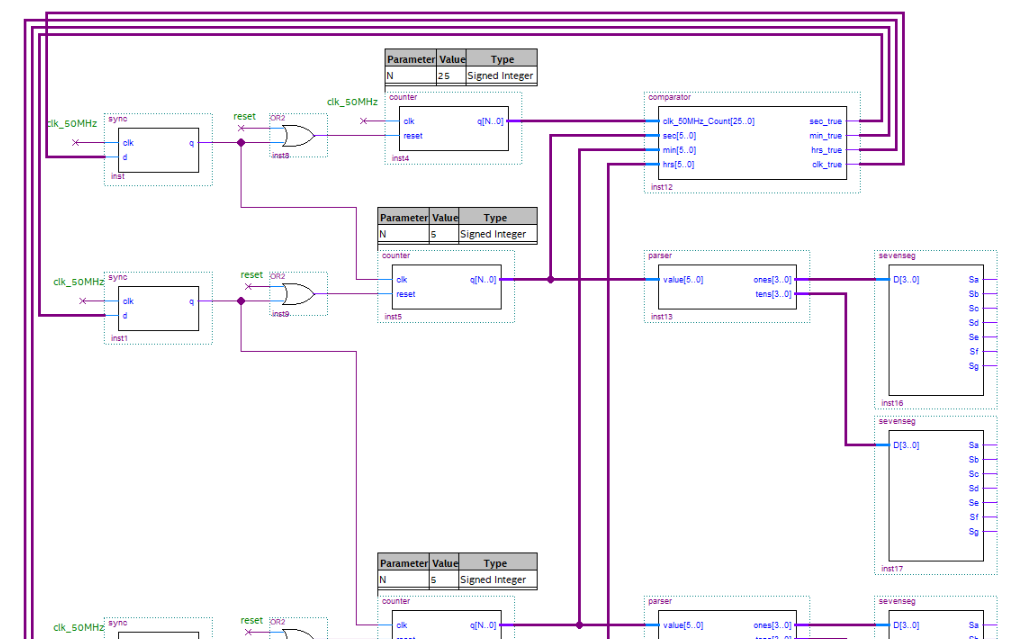
\includegraphics[width=1\linewidth]{png/lab5_block.png}
  \caption{Partial Schematic for Clock}  
\end{figure}.

The basic design structure of the clock is based on utilizing the DE10-Lite's 50MHz clock. The clock serves as an input to the initial counter module, incrementing its output at every positive edge of a clock cycle. This output is then passed into the comparator module. For the initial counter input, the comparator checks if the value has reached 50,000,000. Since the clock operates at 50 MHz, one second elapses for every 50,000,000 clock cycles. If the comparator determines that 50,000,000 cycles have elapsed, it outputs true, which is received by the sync module.

The sync modules act as gatekeepers, ensuring that each counter receives the appropriate clock pulse simultaneously. This output resets the associated counter, preventing it from incrementing beyond the allowed output values. The initial counter has a limit of 50,000,000, while the seconds and minutes counters have a limit of 60, and the hour counter has a limit of 24.

The counter outputs for seconds, minutes, and hours are received by the parser module. The parser evaluates the numbers and outputs the appropriate values to illuminate the corresponding segments of the seven-segment displays. When all the components are connected, a working clock is displayed on the DE10-Lite, presenting the time in military format. The completed SystemVerilog code can be viewed in Appendix 1. All pin assigments were accomplish by importing the Lab5.qsf pin assignment file.

\newpage

\section*{\textcolor{mycolor}{Simulation}}
Simulation of the completed design was done using ModelSim. When run the clock digital logic design correctly output the expected values (Figure 2). 

\begin{figure}[H]
  \centering
  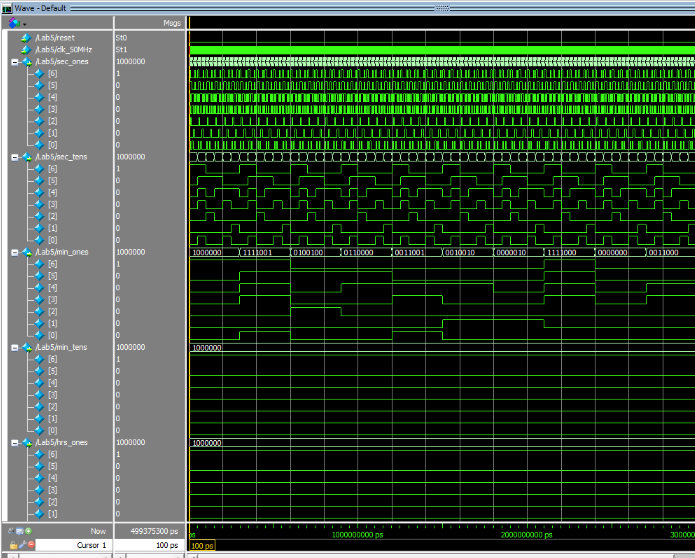
\includegraphics[width=1\linewidth]{png/lab5_sim.png}
  \caption{Partial Simulation for Clock}  
\end{figure}.

\vspace{5mm}
\hrule

\section*{\textcolor{mycolor}{Implementation}}
Implementation in hardware was successful. Each seven segment display incremeneted as expected without errors.

\vspace{5mm}
\hrule

\section*{\textcolor{mycolor}{Observations}}

This lab demonstrated that using SystemVerilog to implement digital logic designs made the process far more streamlined and easier to debug. Text editting offers an increased level of precision and speed of programming that mouse based block diagram construction does.

\vspace{5mm}
\hrule

\section*{\textcolor{mycolor}{Conclusion}}
This lab highlighted the advantages of using SystemVerilog to design and implement digital logic circuits, specifically in the context of creating a clock. By utilizing SystemVerilog, the process of describing and simplifying complex logic became more streamlined and easier to debug compared to traditional schematic-based approaches. The ability to write code provided increased precision and speed in programming.

The successful simulation of the clock design using ModelSim confirmed the expected output values, demonstrating the accuracy of the digital logic implementation. The hardware implementation also proved successful, with each seven-segment display incrementing as expected without errors.

Overall, this lab reinforced the benefits of using SystemVerilog for digital logic design, emphasizing the improved efficiency and ease of debugging. By gaining hands-on experience with SystemVerilog, students enhance their ability to design intricate digital logic circuits effectively.

\vspace{5mm}
\hrule

\section*{\textcolor{mycolor}{Study Questions}}
\subsection*{\textcolor{mycolor}{1. Describe the operation of your Parser.}}
The Parser module works by taking in the input value and performs two operations. First it parses what the ones value is by taking the value modulo 10. In other words it divides the value by ten and assigns the remaining value to the ones variable. 

Then, to find the appropriate tens digit, it takes the value, substracts the value for ones and then divides that by ten. The result is the digit in the tens place. These two values are then outputed to the sevenseg module which will appropriately display the corresponding digit on the display.

\subsection*{\textcolor{mycolor}{2. What does the Synchronizer do and why might it be a good idea to use it?}}

The Synchronizer module is designed to keep each counter in sync. If the synchronizers were not used one counter might increment at before another causing the clock to not display the proper time.

\subsection*{\textcolor{mycolor}{3. How off is your clock?}}
Since each counter must do a comparator check to before sending an update to each sections synchronizer there is an extra clock cycle that takes place. This means the clock will run approximately one clock cycle slower. This can be mitigated by reducing the initial clock comparator value from 50,000,000 to maybe one less, 49,999,999.
\newpage
\section*{\textcolor{mycolor}{Appendix}}
\begin{lstlisting}
  module Lab5( 
    input logic reset,
    input logic clk_50MHz,
      
    output logic [6:0] sec_ones,
    output logic [6:0] sec_tens,
    output logic [6:0] min_ones,
    output logic [6:0] min_tens,
    output logic [6:0] hrs_ones,
    output logic [6:0] hrs_tens
    );
    
    // Main Clock Logic
    
    // counter_clk
    logic clk_50MHz_count;
    logic clk_reset;
    logic [25:0] clk_count;
    
    // clk_sync
    logic clk_true;
    logic clk_true_out;
    
    
    // Seconds Logic
    
    // sec_sync
    logic sec_true;
    logic sec60_true_out;
    
    // sec_counter
    logic [5:0] sec_count;
    
    // sec_parser
    logic [3:0] sec_ones_parser_out;
    logic [3:0] sec_tens_parser_out;
    
    
    // Minutes Logic
    
    // min_sync
    logic min_true;
    logic min60_true_out;
    
    // min_counter
    logic [5:0] min_count;
    
    // min_parser
    logic [3:0] min_ones_parser_out;
    logic [3:0] min_tens_parser_out;
  
    
    // Hours Logic
    
    // hrs_sync
    logic hrs_true;
    logic hrs24_true_out;
    
    // hrs_counter
    logic [5:0] hrs_count;
  
    // hrs_parser
    logic [3:0] hrs_ones_parser_out;
    logic [3:0] hrs_tens_parser_out;
    
  
    // Assignments
    assign clk_reset = reset | clk_true_out;
    assign sec_reset = reset | sec60_true_out;
    assign min_reset = reset | min60_true_out;
    assign hrs_reset = reset | hrs24_true_out;
    
  ///////////////////////////////
    
    sync clk_sync(
      .clk(clk_50MHz),
      .d(clk_true),
      .q(clk_true_out));
      
    counter #(25) clk_counter(
      .clk(clk_50MHz),
      .reset(clk_reset),
      .q(clk_count));
      
    comparator clk_comparator(
      .clk_50MHz_Count(clk_count),
      .sec(sec_count),
      .min(min_count),
      .hrs(hrs_count),
      .sec_true(sec_true),
      .min_true(min_true),
      .hrs_true(hrs_true),
      .clk_true(clk_true));
    
  ///////////////////////////////
  
    sync sec_sync(
      .clk(clk_50MHz),
      .d(sec_true),
      .q(sec60_true_out));
    
    counter #(5) sec_counter(
      .clk(clk_true_out),
      .reset(sec_reset),
      .q(sec_count));
    
    parser sec_parser(
      .value(sec_count),
      .ones(sec_ones_parser_out),
      .tens(sec_tens_parser_out));
    
    sevenseg sec_ones_disp(
      .D(sec_ones_parser_out),
      .Sa(sec_ones[0]),
      .Sb(sec_ones[1]),
      .Sc(sec_ones[2]),
      .Sd(sec_ones[3]),
      .Se(sec_ones[4]),
      .Sf(sec_ones[5]),
      .Sg(sec_ones[6]));
    
    sevenseg sec_tens_disp(
      .D(sec_tens_parser_out),
      .Sa(sec_tens[0]),
      .Sb(sec_tens[1]),
      .Sc(sec_tens[2]),
      .Sd(sec_tens[3]),
      .Se(sec_tens[4]),
      .Sf(sec_tens[5]),
      .Sg(sec_tens[6]));
    
  ///////////////////////////////
    
    sync min_sync(
      .clk(clk_50MHz),
      .d(min_true),
      .q(min60_true_out));
    
    counter #(5) min_counter(
      .clk(sec60_true_out),
      .reset(min_reset),
      .q(min_count));
      
    parser min_parser(
      .value(min_count),
      .ones(min_ones_parser_out),
      .tens(min_tens_parser_out));
    
    sevenseg min_ones_disp(
      .D(min_ones_parser_out),
      .Sa(min_ones[0]),
      .Sb(min_ones[1]),
      .Sc(min_ones[2]),
      .Sd(min_ones[3]),
      .Se(min_ones[4]),
      .Sf(min_ones[5]),
      .Sg(min_ones[6]));
    
    sevenseg min_tens_disp(
      .D(min_tens_parser_out),
      .Sa(min_tens[0]),
      .Sb(min_tens[1]),
      .Sc(min_tens[2]),
      .Sd(min_tens[3]),
      .Se(min_tens[4]),
      .Sf(min_tens[5]),
      .Sg(min_tens[6]));
    
  ///////////////////////////////
  
    sync hrs_sync(
      .clk(clk_50MHz),
      .d(hrs_true),
      .q(hrs24_true_out));
    
    counter #(5) hrs_counter(
      .clk(min60_true_out),
      .reset(hrs_reset),
      .q(hrs_count));
      
    parser hrs_parser(
      .value(hrs_count),
      .ones(hrs_ones_parser_out),
      .tens(hrs_tens_parser_out));
    
    sevenseg hrs_ones_disp(
      .D(hrs_ones_parser_out),
      .Sa(hrs_ones[0]),
      .Sb(hrs_ones[1]),
      .Sc(hrs_ones[2]),
      .Sd(hrs_ones[3]),
      .Se(hrs_ones[4]),
      .Sf(hrs_ones[5]),
      .Sg(hrs_ones[6]));
    
    sevenseg hrs_tens_disp(
      .D(hrs_tens_parser_out),
      .Sa(hrs_tens[0]),
      .Sb(hrs_tens[1]),
      .Sc(hrs_tens[2]),
      .Sd(hrs_tens[3]),
      .Se(hrs_tens[4]),
      .Sf(hrs_tens[5]),
      .Sg(hrs_tens[6]));
    
  endmodule  
\end{lstlisting}

\begin{lstlisting}
  module parser(
    input logic [5:0] value, 
    output logic [3:0] ones, tens);
    
    always_comb
    
    begin
    ones = value % 10;
    tens = (value - ones)/10;
    end
    
    endmodule
    
\end{lstlisting}

\end{document}